\section{Approach}
\label{sec:approach}


In this section, we first formalize the commonsense reasoning classification problem
and then introduce our three noise data augmentation methods.
 
\subsection{Problem Statement}
\label{sec:problem_statement}
We define an instance $x$ of a natural language reasoning task 
dataset $X$ as
\begin{equation}
    x = (p, h, r) \in X, \label{eq:nli}
\end{equation}
\noindent
where $p$ is the context against which to do the reasoning ($p$ corresponds 
to ``premise'' in~\figref{fig:example});
$h$ is the hypothesis given the context $p$; 
$r \in \mathcal{R}$ is the label that 
depicts the type of relation between $p$ and $h$. 
%Given a natural language
%premise $p$ and a hypothesis $h$, we should judge the 
%relation from the alternative label set $L$ between $p$ and $h$. 
In FEVER, the \textit{evidence} corresponds to the premise and the 
\textit{claim} is a hypothesis based on \textit{evidence}. 
%For the shallow spurious features, like 
%unbalanced word distribution, word overlap and hypothesis-only, misleading models to
%learn reasoning unrelated features and affecting models' robustness, 
%our goal is to generate noisy data to weaken these features and improve 
%the reasoning ability of models.
% The reason we design noises this way is that we aim to avoid
%introducing new spurious cues into original task. Even if models learn the spurious
%features in the new ``Noise'' examples, it won't give extra spurious information
%for reasoning test (test without label ``Noise''). This is inspired by the thinking of joint learning.
%Together with the original examples of the dataset, we come up with an augmented dataset
%which we call noise dataset.

\subsection{Noise Data Augmentation Methods}
\label{sec:noise_methods}

If a model is shown to be fragile by the adversarial tests, its performance
may decline, especially when applied to out-of-distribution
test data. To make models more robust, one natural 
thought is to generate more data to encourage models to
focus on the relation between the premise and choices. Intuitively,
noise data augmentation is utilized to optimize
the model by increasing the difficulty of training so that the model cannot be easily
fit with shallow spurious cues and pay more attention to the relationship between the 
premise and hypothesis. We weaken the impacts of spurious cues with three kinds of noise: 
balanced distribution noise, overlap noise and hypothesis-only noise. 
%We give 3 examples 
%for each noise type in~\figref{fig:}

\subsubsection{Balanced Distribution Noise}

\begin{figure}[th!]
	\centering
	\includegraphics[width=0.6\columnwidth]{figures/noise_balance.eps}
	\caption{The frequency of some words sampled from SNLI which mostly appears in Contradiction labeled examples.
	}
\label{fig:noise_balance}
\end{figure}

Since the n-gram cues distribution based on the label can be one reason for 
model failure on adversarial tests, we statistic the frequency of 
each token based on different labels and observe disparities in distribution. 
It is noted that we only consider single-word tokens in this paper which is also widely mentioned 
in others' work~\cite{niven2019probing,naik2018stress}. 
In~\figref{fig:noise_balance}, we only sample 10 single words 
which always appear in ``Contradiction'' of SNLI, 
for example, the word ``nobody'' almost never appears 
in ``Entailment'' and ``Neutral'' instances which may misguide models to choose 
``Contradiction'' once they find ``nobody'' in an instance. Except for 
some ``negative'' adjectives and adverbs, many nouns like ``cat'' and ``couch'' 
are also highly unbalanced. In order to eliminate the serious disparities, 
we propose to ``flatten'' the distribution of each word $w$ in a vocabulary 
set $V$ of the dataset by adding 
new instances with the label ``Noise''. The appearance of word $w$ with the label ``Noise'' 
should be equal to the maximum number of word $w$ co-occurence with one label $r$. 
The frequency of word $w$ based on label $r_{i}\in{R}$ is denoted as $freq(w, r{i})$. 
The number of words which should be appeared in ``Noise'' data is calculated as bellow
%\YZ{The write style of Noise in function has some problem}:

 \begin{equation}
    freq(w, ``Noise'') = \max(freq(w, r_{i}), r_{i}\in{R} \wedge r_{i}\neq{``Noise''}
\end{equation}

Then, we aggregate all the words which should be appeared in 
noise data as $W$ and generate new instances by random sample words from $W$ with 
an average length of the premise and hypothesis which doesn't conform grammar. 
The number of new instances is $\frac{|W|}{\bar{|p|}+\bar{|h|}}$.

\subsubsection{Overlap Noise}

\begin{figure}[th!]
	\centering
	\includegraphics[width=\columnwidth]{figures/noise.eps}
	\caption{Overlap noise example and hypothesis-only example.}
\label{fig:noise2and3}
\end{figure}

Overlap noise is illustrated in \figref{fig:noise2and3}, and 
we take the same example with~\cite{mccoy2019right}.
A model that labels the example correctly
might do not by reasoning about the relation
of these sentences, but rather by assuming that the
premise entails any hypothesis whose words mostly 
appear in the premise. Given a new premise ``The actor was paid by the judge'', 
the model may still predict ``Entailment'' if it only learns the overlap spurious features,
even though the correct label is changed to contradiction. 
To reduce the influence of overlap cues, we generate 
noise cases with a new premise by randomly choosing some words from the hypothesis and preserving the hypothesis. 
We fill in the premise with other words which are different from the chosen ones to maintain 
the length of the premise with $|p|$. The noise example(1) in~\tabref{fig:noise2and3} shows 
a corresponding overlap instance we generate. The premise isn't grammatical.


\subsubsection{Hypothesis-only Noise}

%Hypothesis-only noise is illustrated in \figref{fig:noise2and3} example(2). 
Due to the limited interpretability of deep neural models,
the hypothesis-only test is used as one kind of interpreter for models. 
%the whether the models can 
%get very high accuracy score without given premise. 
%This kind of test is called hypothesis-only test. 
For example, BERT, when
fine-tuned on the SNLI data, can answer the question in the original NLI example 
in \figref{fig:noise2and3} correctly. 
When we remove the premise from the
same question and feed it to the model, 
it still gets the correct
answer (``Entailment''). 
This result from the hypothesis-only
test seems to suggest that the model can make correct predictions
without even looking at the premise. 
%As the name indicates, the premise is a null string. For example, in~\tabref{fig:noise2and3} 
To encourage models to pay more attention to the relationship between premise and hypothesis, 
we generate noise cases with a null string premise and the hypothesis in the original example. 
Hypothesis-only noise is illustrated in \figref{fig:noise2and3} example(2). 
%noise example(2), we cannot predict the commonsense reasoning relation with a single component obviously. 
%Thus this kind of information is also noisy data. 

\subsection{Loss}
\label{sec:loss}
%\KZ{WHen you say ``system'', did you mean ``model?'' System usually has a diff
%meaning. Be consistent.}
Our data augmentation methods don't change the original datasets and model structure. 
In fact, we enhance the model by changing the loss function implicitly. The label set is 
$R=(Ent., Con., Neu.)$.
The original loss function can be expressed as:
 \begin{equation}
 	loss = -\sum_{i}^{R}t_{i}\log s_{i}=-\left ( t_{Ent.}\log s_{Ent.} + t_{Con.}\log s_{Con.} +  t_{Neu.}\log s_{Neu.}\right )
    %freq(w, ``N = \max(freq(w, l_{i}), l_{i}\in{L} \wedge l_{i}\neq{``Noise''}
\end{equation}
Each sample can belong to one of  $R$ classes.
 The neural model will output probability for $|R|$ classes that can be gathered in a vector $s$, 
The target (ground truth) vector $t$ will be a one-hot vector with a positive class and $|R|-1$ negative classes.

Training with our augmentation datasets, the new label set is: 
%\begin{equation}
$R^{'}=(Ent., Con., Neu.,\\ Noise)$.
%\end{equation}
The loss function can be expressed as:

\begin{equation}
\begin{aligned}
 loss &= -\sum_{i}^{R^{'}}t_{i}\log s_{i} \\
      &=-\left ( t_{Ent.}\log s_{Ent.} + t_{Con.}\log s_{Con.} +  t_{Neu.}\log s_{Neu.} +  t_{Noise}\log s_{Noise}\right )
    %freq(w, ``Noise'') = \max(freq(w, l_{i}), l_{i}\in{L} \wedge l_{i}\neq{``Noise''}
\end{aligned}
\end{equation}

















